\documentclass[12pt]{article} % Clase de documento, tamaño de letra 12pt

% Paquetes importantes
\usepackage[utf8]{inputenc}   % Codificación de entrada UTF-8 para caracteres acentuados
\usepackage[T1]{fontenc}      % Codificación de salida para que el texto se vea bien en PDF
\usepackage[spanish]{babel}   % Traduce términos automáticos al español (ej. "Figura", "Resumen")

\usepackage{csquotes}         % Recomendado para manejar comillas y citas con biblatex
\usepackage{graphicx}         % Permite incluir imágenes con \includegraphics
\usepackage{setspace}         % Para controlar interlineado; APA pide interlineado doble
\usepackage{geometry}         % Controla los márgenes de la página (APA pide 1 pulgada = 2.54cm)
\usepackage[hidelinks]{hyperref}        % Habilita enlaces clicables en el PDF (tabla de contenido, referencias)
\usepackage[style=apa, backend=biber]{biblatex}  % Bibliografía con estilo APA 7 y gestor biber
\addbibresource{referencias.bib}  % Archivo con las referencias bibliográficas (formato .bib)

% Carga tu paquete personalizado que contiene el comando \imprimircaratula
\usepackage{caratula}

%para decorar el indice
\usepackage{tocloft} %Conectar los títulos con los números de página usando puntos
\renewcommand{\cftsecleader}{\cftdotfill{\cftdotsep}} %Esto añadirá los "........" entre el título y la página.
\setcounter{tocdepth}{4}   % incluye paragraph en la ToC
\setcounter{secnumdepth}{4}% (opcional) numera hasta paragraph

% Define los márgenes recomendados por APA: 1 pulgada en todos lados
\geometry{letterpaper, margin=1in}

% Permite personalizar el formato de títulos (secciones y subsecciones)
\usepackage{titlesec}
% Define estilo para títulos de sección: tamaño grande y negrita
\titleformat{\section}{\normalfont\large\bfseries}{\thesection}{1em}{}
% Define estilo para títulos de subsección: tamaño normal y negrita
\titleformat{\subsection}{\normalfont\normalsize\bfseries}{\thesubsection}{1em}{}

% Define interlineado doble, que es requerido por APA
\doublespacing

%para la tabla
\usepackage{pdflscape} %Para rotar la página
\usepackage{adjustbox} %Para redimensionar automáticamente el contenido
\usepackage{tabularx} %Para hacer que la tabla ocupe todo el ancho de la página usando columnas flexibles
\usepackage{array} % Para usar >{\centering\arraybackslash}
\usepackage[table,xcdraw]{xcolor} %Para darle color al encabezado
\definecolor{headerbg}{HTML}{D9E1F2} % Para definir un color de encabezado
\usepackage{multirow}      % Para combinar filas

%para personalizar el header
\usepackage{fancyhdr}           % Para encabezados y pies personalizados
\pagestyle{fancy}               % Activar fancyhdr para todas las páginas
\fancyhf{}                      % Limpia encabezados y pies por defecto
\fancyhead[L]{J. Aulla; M. Millan} % Encabezado a la izquierda con las siglas
\fancyhead[R]{\thepage}
\renewcommand{\headrulewidth}{0pt} %quita la linea debajo de los nombres y numero de pagina

%para anexo
\usepackage{tocloft}



% Datos para título, autor y fecha (aunque no se usan porque tienes portada personalizada)
\title{Título del Documento en Formato APA 7}
\author{Nombre del Autor}
\date{\today}

%-----------------------------------------------------------------------------------
%inicio del documento
%-----------------------------------------------------------------------------------



\begin{document}

% Imprime la portada con el comando definido en tu paquete caratula.sty
\imprimircaratula

\begin{center}
    \vspace*{3cm} 
    \normalsize \textbf{DEDICATORIA} 
    \vspace{6cm}
\end{center}
\hspace{7.9cm}
\begin{minipage}{\dimexpr\textwidth-8cm}
    \textcolor{gray}{
        Le dedicamos este trabajo a nuestros familiares, amigos y compañeros, 
        quienes nos han ayudado a alcanzar nuestros objetivos, apoyándonos y 
        aconsejándonos en circunstancias poco favorables.
    }
\end{minipage}

\newpage

\begin{center}
    \vspace*{3cm} 
    \normalsize \textbf{AGRADECIMIENTOS} 
    \vspace{6cm}
\end{center}
\hspace{7.9cm}
\begin{minipage}{\dimexpr\textwidth-8cm}
    \textcolor{gray}{
        Expresamos nuestro sincero agradecimiento a nuestra docente guía, \textbf{Mg. Anita Cando López}, por su constante apoyo, orientación y dedicación durante el desarrollo de este proyecto.
    }
\end{minipage}

\newpage

% Tabla de contenidos automática
\tableofcontents
\newpage

\newlistof{listanexfig}{anx}{Índice de anexos de imágenes}


% Resumen (abstract) con su propio entorno
\begin{abstract}

\end{abstract}
\newpage

% Sección Introducción
\section*{\makebox[\linewidth][c]{Introducción}}
\addcontentsline{toc}{section}{Introducción}
\setcounter{section}{1}
\newpage




% Inicio del primer Capítulo
\section*{\makebox[\linewidth][c]{Capítulo I}}
\addcontentsline{toc}{section}{Capítulo I}




% Definición del Problema
\subsection{Definición del Problema}

\subsubsection{Descripción del Problema}

Los almacenes clínicos resguardan y controlan los diferentes insumos y reactivos para su posterior uso. dichos almacenes deben poder registrar por lotes, fecha de vencimiento y tener conservación bajo normas de seguridad. Por lo que, a nivel mundial cuando la gestión de inventarios carece de esta estandarización y automatización se producen diferentes problemas como el sobrestock, vencimiento de reactivos, diferencia entre los registros en los sistemas y lo físico, lo que eleva los costos y compromete la continuidad operativa.

según Odoñez y Bustillo(2024), en el caso de LACM el control se realiza periodicamente pero con procesos aún manuales, detectando discrepancias entre inventario en sistema y físico, y por ello intentaron implementar un sistema formal con políticas claras y herramientas de gestión para reducir mermas y evitar el desabastecimiento.

En Latinoamérica, muchos laboratorios clínicos aún gestionan insumos y reactivos con planillas de Excel y procesos manuales. Esto dificulta el seguimiento de lotes y fechas de caducidad, ralentiza la búsqueda de información y eleva el riesgo de desabastecimiento, afectando la calidad y la oportunidad del servicio (según Rivera Silva,2024).

de igual manera, en Ecuador, el laboratorio IN VITRO (cantón Pajan) trabaja con Word/Excel y facturacion manual, lo que entorpece el control de existencias y de caducidades. Las encuestas a 152 pacientes muestran que el 92\% considera necesaria la implementación de un sistema informático para gestionar inventarios y facturación, el 95\% cree que reduciría los tiempos de espera y el 79\% piensa que mejoraría la calidad de la atención (según Rivera Silva, s.f.).

En el contexto peruano, los laboratorios clínicos deben operar bajo lineamientos de calidad que exigen gestión documentada de procesos, personal calificado y control de insumos y reactivos (ISO/CLSI) y normas peruanas como la NTS N.° 072-MINSA y la NTP-ISO 15190, lo que vuelve crítica la administración del inventario para asegurar continuidad del servicio y seguridad del paciente (Alvarado, 2023). Como consecuencia, la ausencia de un sistema funcional para el control del almacén puede resultar en múltiples problemas, tales como el no conocimiento sobre el momento oportuno para reabastecer reactivos, la interrupción de actividades por escasez de insumos en el laboratorio, así como también en complicaciones legales y pérdidas económicas.

\subsubsection{Formulacion del Problema}

\paragraph{Problema General}%\mbox{}\\[0.5ex]     <b    nk jg

¿Cómo lograr un control eficiente de los reactivos en el almacén de un laboratorio clínico?

\paragraph{Problemas especificos}

\begin{itemize}
    \item Tiempo de búsqueda de la información excesivos.
    \item Errores en el registro de ingreso y salida de reactivos.
    \item Falta de conocimiento del stock actual.
    \item Acceso a la información limitada.
    \item Falta de seguimiento de productos por vencer.
\end{itemize}

\subsection{Definicion de Objetivos}

\subsubsection{Objetivo General}

Desarrollar una Solución Web para gestionar el inventario de laboratorio clínico.

\subsubsection{Objetivos Especificos}

\begin{itemize}
    \item Agilizar la búsqueda de información.
    \item Controlar el registro de datos para evitar errores de diversa índole.
    \item Gereración de Reportes del stock actual.
    \item Permitir el acceso de la informacion desde cualquier lugar.
    \item Emitir alertas para productos por caducar.
\end{itemize}



\subsection{Alcances y Limitaciones}

\subsubsection{Alcances}

El sistema se implementará como una aplicación web responsive, accesible desde cualquier navegador con conexión a internet. Además, la interfaz priorizará la usabilidad y la experiencia del usuario, asegurando que las funciones principales sean intuitivas y fáciles de usar como tareas frecuentes (consultas, salidas y registros) y contará con autenticación y roles básicos para un acceso controlado.

La información se concentrará en un repositorio único que incluirá catálogo de productos, lotes, fecha de caducidad y movimientos internos. Por lo que, cada operacion registrará los tiempos y usuarios responsables para asegurar trazabilidad y disminuir inconsistentecias. Esta centralización lograra establecer una fuente confiable de los datos, fortaleciendo la integridad y la calidad de la información.

El sistema generará reportes de inventario vigente por producto, lote, ubiación y cantidad de unidades disponibles. Por lo que, se presentarán indicadores clave como el stock mínimo y variaciones recientes, a fin de respaldar decisiones de reabastecimiento y control operativo. 

\subsubsection{Limitaciones}

El sistema gestionará el inventario de un único almacén. No contemplará transferencias intersede ni reportes centralizados multisucursales

El acceso del sistema será exclusivamente para navegadores web. Por lo que, no se permitirá el acceso por otros medios como Apps Android o iOS.

No se prevé un modo sin conexión. Por lo que, las operaciones de las consultas y registros nesecitarán conectividad a una red de internet.

\subsection{Justificación}

\subsubsection{Economico}

El sistema impacta directamente en los costos del laboratorio al disminuir pérdidas por caducidad de los reactivos. Debido a que, la gestión por lotes y fechas, apoyada por alertas tempranas, permitirá priorizar el uso de insumos próximos a vencer y planificar su consumo o redistribución. Con lo mencionado, se logrará reducir gastos de disposición de residuos y compras no previstas.

Asimismo, el sistema proveerá información oportuna para la toma de decisiones. Ya que, los reportes proporcionados logrará evitar situaciones como la quiebra de stock como el sobreinventario.

\subsubsection{Tecnologico}

Al implementar una plataforma web moderna, con interfaz responsive, control de acceso por roles y trazabilidad de operaciones situará al laboratorio por encima de los esquemas básicos. Por lo que, se adoptaría buenas prácticas de seguridad y auditoría y por consiguiente mejorará la confiabilidad operativa, reforzará una imagen de modernización frente a los clientes.

Adicionalmente, el sistema se diseñará con una arquitectura modular, preparada para crecer sin reescrituras. Por lo que, este enfoque facilita incorporar, en siguientes fases, múltiples mejoras para el sistema.


\subsubsection{Social}

Al ser una aplicación accesible desde cualquier navegador web con conexión a internet, el personal podrá consultar existencias, registrar movimientos y gestionar vencimientos sin depender de estar ubicado físicamente en el almacén. esto mejorará la coordinación entre todo el personal encargado del almacen.

\subsubsection{Ambiental}

Al digitalizar todas las actividades de la gestión del almacén, se evitará el uso de cuadernos, hojas, impresiones y materiales de oficina. Por lo que, se logrará reducir la producción de residuos sólidos y la huella asociada a la produccion de papel y consumibles.

\section*{\makebox[\linewidth][c]{Anexos}}
\addcontentsline{toc}{section}{Anexos}



\begin{figure}[h]
    \centering
    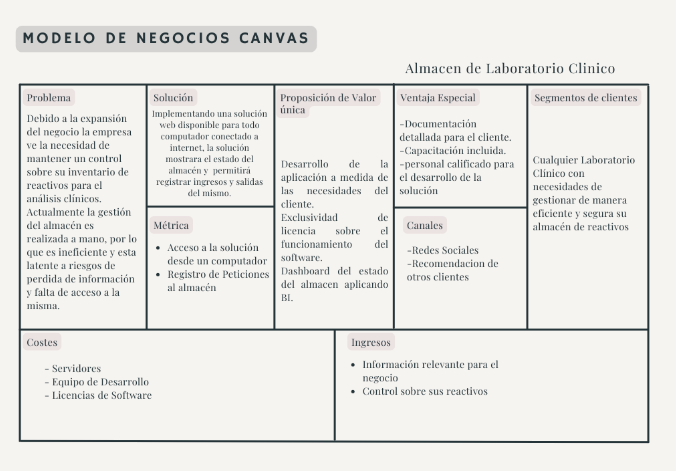
\includegraphics[width=1\textwidth]{Lean Canvas.png} % Imagen de ejemplo que viene con distribuciones LaTeX
    \caption{Lean Canvas que difine el proyecto}
    \label{fig:imagen_ejemplo} % Etiqueta para referenciar la imagen en texto
\end{figure}


\end{document}
